\documentclass{llncs}
%\usepackage{fancyhdr}
\pagestyle{plain}
%\pagestyle{headings}
\usepackage{standalone}
\usepackage{graphicx} 
\usepackage{comment}
%\usepackage{xcolor}
\usepackage{epigraph}
\usepackage{amsmath}
\usepackage{amsfonts}
\usepackage{amssymb}
%\usepackage{natbib}
%\usepackage[title]{appendix}
\usepackage{caption}
\usepackage{subcaption}
\usepackage{latexcolors}
\usepackage{import}
\usepackage{tikz}
\usetikzlibrary{positioning}
\usetikzlibrary {arrows.meta}


\begin{document}

%


\title{Telling the story of best friends}
%
\titlerunning{Best friends}  
% abbreviated title (for running head)
%                                     also used for the TOC unless
%                                     \toctitle is used
%
\author{
Alexandra Suvorikova \inst{1} \and Vasiliy Ramensky \inst{2} \and Vera Mukhina \inst{3} 
\and Andrey Mironov \inst{4} \and Alexander Favorov\inst{5}\textsuperscript,\inst{6}}
%
\authorrunning{A. Suvorikova et al.} % abbreviated author list (for running head)
%
%%%% list of authors for the TOC (use if author list has to be modified)
\tocauthor{Alexandra Suvorikova, Vasiliy Ramensky, Vera Mukhina, Andrey Mironov, and Alexander Favorov}
%
\institute{
Weierstrass Institute, \\ Berlin, Germany, 
\email{suvorikova@wias-berlin.de}
\and
National Health and Research Center of Preventive Healthcare, \\ Moscow, 101990, Russia
\and
University of Maryland School of Medicine, \\ Baltimore, MD 21205, USA,
\and
Department of Bioengineering and Bioinformatics, MSU, \\ Moscow, 119992, Russia
\and
Johns Hopkins University School of Medicine, \\ Baltimore, MD 21205, USA,
\and
Vavilov Institute of General Genetics, RAS, \\ Moscow, 119333, Russia, 
\email{favorov@sensi.org}
}

\maketitle              % typeset the title of the contribution

\renewcommand{\tag}{tag}
\newcommand{\collection}{collection}
\newcommand{\T}{T}
\newcommand{\C}{C}
\newcommand{\tl}{t}
\newcommand{\cl}{c}
\newcommand{\test}[1]{\textbf{\textit{#1}}}
%\setlength\epigraphwidth{.8\textwidth}
\setlength\epigraphrule{0pt}

\epigraph{SI AUGUSTUS CERNATUR, CERNANTUR QOUQUE AMICI}

\vspace{-0.2in}

\begin{abstract}

\textcolor{green}{We define a tag's most friendly collection as a collection that pays maximal rank-normalized attention to the tag.}
\textcolor{blue}{ -- we will return here --} \textcolor{purple}{
Suppose we have a set of {\tag}s and a set of fuzzy set of {\tag}s, which we will refer to as {\collection}s, and we have the {\tag}-to-{\collection} relation quantified as a scalar for each $\left( {\tag},{\collection}\right)$ pair. An example is: {\tag}s are genes, {\collection}s are gene expression patterns, and the scalars are loads of the genes in the patterns. Sometimes, an observation that a gene is expressed implies the expression of a particular pattern (the simplest case is: the gene has nonzero load only in that pattern). If so, we say that the gene marks the pattern. Here we describe a statistical test that identifies pairs of a marker {\tag} and the marked {\collection}. The test is based on rank statistics and it does not rely on propositions about the distribution of the relation quantity. The marked {\collection} is referred to as the {\tag}'s best friend, and the test is named "the best friends test" or "the gene's best friends test". The statistics naturally expand to the case when a {\tag} selects (separates) a subset of {\collection}s, thus having more than one best friend. The code (currently, only R) is available at \url{https://github.com/favorov/best-friends}
\keywords{best friends, gene's best friends, specific gene regulation, pattern marker, rank statistics, marker feature, marked entity}
}
\end{abstract}
%
\section{Introduction: Augustus and his friends}

There is a simple intuition of what does it mean to be a friend. A friend of Augustus cares about Augustus more than other people do. And, if we see Augustus, then we infer to see friends(s) of Augustus also. 

Let's introduce the friendship concept with several examples.
The first example comes from information retrieval. The goal is to find the documents that are most relevant to the user's query among all available documents \cite{liu2009learning}. 

In the second example, we consider a set of genes and their loads in a set of expression patterns (\cite{fertig_cogaps_2010,Fertig_2016,stein-obrien_enter_2018}). Each pattern represents a biological process by the expression levels of the involved genes, and we know all the loads of genes in patterns.

Sometimes, the expression of a single gene indicates the activity of the entire pattern. In the simplest case, the gene has a nonzero load in only one pattern. In more realistic, the gene has several nonzero loads, but all of them but one are relatively small. Then the gene (AKA Augustus) is the marker gene \cite{stein-obrien_patternmarkers_2017} for the pattern, and the marked pattern is the best friend of this gene. We want to identify the marker genes and corresponding patterns statistically.  


The third example deals with gene-to-gene correlation matrix (e.g. correlation of expression). High correlation indicates high similarity between genes. For a given gene, the goal is to indicate its ``best-friend'' genes among genes. \textcolor{red}{examples????}


The bipartite graph suits well to describe the problem setups. To generalise the examples, we will refer to genes/queries as \textit{{\tag}s}, to expression patterns/documents as \textit{{\collection}s}, and to any load/relevance value as \textit{attention}. Of note, the attention is the weight of an edge connecting a tag and a collection. Fig.\ref{fig:nice_name} illustrates the setting.

\begin{figure}
    \centering
    %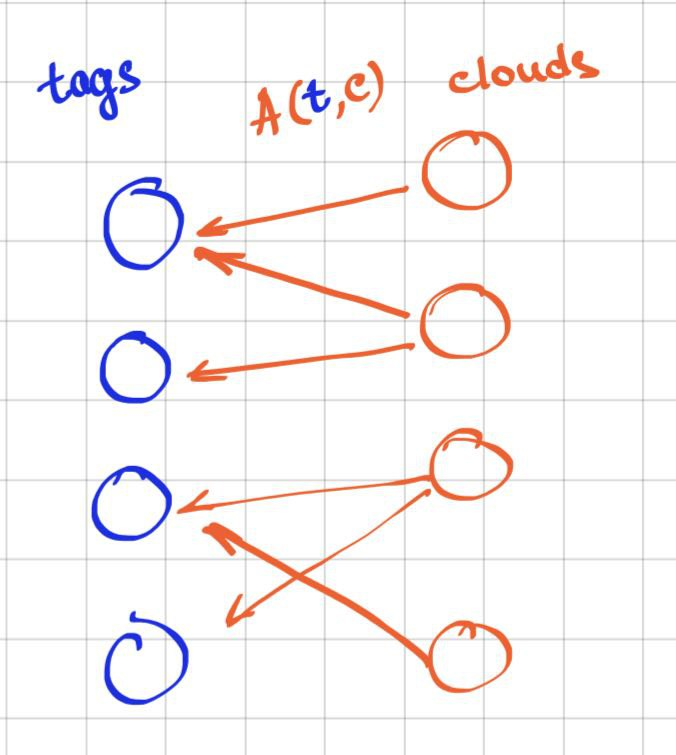
\includegraphics[scale=.25]{bipartite.jpg}
    \import{}{bipartite}
    \caption{Bipartite graph presenting tag-collection model. $A(t,c)$ is the attention that a collection pays to a tag. Arrows are nonzero $A(t,c)$.}
    \label{fig:nice_name}
\end{figure}

To be more specific, we consider a set of collections $C = \{c_1, \dots, c_k\}$, and a set of tags $T = \{t_1, \dots, t_n\}$.
Each tag $t_i \in T$ and collection $c_j \in C$ are related by the attention---the real value $a_{ij}$---that the collection pays to the tag.
Let's agree that the greater the value, the higher the attention is. Naturally, the absence of attention corresponds to $a_{ij} = 0$. 

All the values $a_{ij}$ are stored in a matrix $\mathcal{A}$; its row $\mathcal{A}_{i:}$ corresponds to tag $t_i$, its column $\mathcal{A}_{:j}$ corresponds to collection $c_j$.

This tag-collection-attention metaphor applies to many setups (see Tab.\ref{tab:examples} for examples).

\begin{table}[h!]
\centering
\begin{tabular}{c|c|c|c}
\textbf{Example} & \textbf{tag $t_i$} & \textbf{collection $c_j$} & \textbf{attention $a_{ij}$} \\ 
\hline

\begin{tabular}[c]{@{}c@{}}search engine\end{tabular} & query       & \begin{tabular}[c]{@{}c@{}} search result \end{tabular}         & \begin{tabular}[c]{@{}c@{}}relevant search output\\\end{tabular} \\ \hline

\begin{tabular}[c]{@{}c@{}}gene regulation\\  by TFs\end{tabular}     & gene             & \begin{tabular}[c]{@{}c@{}}genes under \\ TF regulation\end{tabular}     & \begin{tabular}[c]{@{}c@{}}strength of \\ regulation\end{tabular}       \\ \hline

\begin{tabular}[c]{@{}c@{}}transcription\\ decomposition\end{tabular} & transcript       & \begin{tabular}[c]{@{}c@{}}transcription \\ pattern\end{tabular}         & \begin{tabular}[c]{@{}c@{}}transcript's \\ load in pattern\end{tabular} \\ \hline

\begin{tabular}[c]{@{}c@{}}transcription \\ correlations\end{tabular} & gene             & \begin{tabular}[c]{@{}c@{}}genes coexpressed \\ with a gene\end{tabular} & \begin{tabular}[c]{@{}c@{}}transcription \\ correlation\end{tabular}    \\ \hline
fuzzy clustering                                                      & object           & cluster                                                                  & \begin{tabular}[c]{@{}c@{}}object weight \\ in cluster\end{tabular}     \\ \hline


\begin{tabular}[c]{@{}c@{}}weighted graph\end{tabular} & vertex       & \begin{tabular}[c]{@{}c@{}} another vertex \end{tabular}         & \begin{tabular}[c]{@{}c@{}}weight of edge between\\ collection and tag \end{tabular} \\ \hline


\end{tabular}

\caption{Tag-collection metaphor deployment examples.}
\label{tab:examples}
\end{table}

Let's recall the intuition that starts the introduction. A friend of Augustus cares about Augustus more than other people do. In the following, we depict the concept of care using ranking. Indeed, the ranking approach widely appears in our scope of interest.
Partial or total ranking of documents for a given query is a popular strategy in information retrieval \cite{liu2009learning}. In bioinformatics, many methods rely on ranking, e.g. feature selection \cite{venetis2011selection}, marker selection \cite{vargo2020rank}, \cite{pullin2022comparison}, \cite{jimenez2021multivariate}, etc.

The idea of ranking can be applied in a na\"ive way: the higher the attention of a collection to a tag is, the more friendly the collection is to the tag. But in some cases, this is not enough.

Let's recall the example of gene-to-gene correlation. The na\"ive approach is to fix a gene of interest and rank other genes according to their correlation. This ranking cannot tell between the genes, which specifically correlate with the gene of interest, and the network hub genes (i.e., genes that carelessly correlate with all the genes). 

Therefore, we suggest using double-ranking approach. As any ranking approach, it is distribution-free. Moreover, it allows us to define the concept of friendship via the concept of care in accordance with the Augustus intuition, and thus to point to the most friendly collection for each tag. \textcolor{airforceblue}{Below, we will see how the concept helps us to statistically distinguish between the friends-by-accident and real best friends.}

First, we fix a collection $c_j$ and rank the attention values $a_{1j}, \dots, a_{nj}$. This ranking indicates how much the collection $c_j$ cares about any tag $t_i$. Thus, any collection $c_{j}$ and any tag $t_i$ are connected by the rank $r_{ij}$.

Second, we fix a tag $t_i$ and rank all collections by the tag's ranks in a collection $r_{i1}, \dots, r_{ik}$.
This step expresses the intuition of Augustus numerically: the collection $c_j$ with the highest rank $r_{ij}$ among $r_{i1}, \dots, r_{ik}$ 
 \textcolor{purple}{cares the most about $t_i$ and it }can be the best friend of $t_i$. However, having the highest rank is necessary, but not sufficient to be the real best friend.

Of note, friendship in this notation is a property of the whole matrix $\mathcal{A}$. Thus, the null-hypothesis $H_0$ claiming no friendship at all, consists of assumptions on all the values in $\mathcal{A}$.

Under $H_0$, we assume that the attention values from a cloud $c_j$ to all tags are independent and identically distributed.
This distribution can vary from cloud to cloud. Moreover, all the $n \times k$ attention values $a_{ij}$ from collections to tags are independent.

We suggest a test checking whether $c_j$ is really the best friend of $t_i$ or $c_j$ appears at the top of the ranking by chance (i.e. according to $H_0$). The test is $p$-value based and compares the ordered ranks for $t_i$ in different collections. We name it the \test{best friend test}.

Looking for a possible best friend and statistically assessing the friendship, we start with a data set represented by a bipartite graph of vertices representing tags and collections and edges representing attention from collection to tag.
To start with, we choose a tag and then we look for a collection. As we see, the procedure is asymmetric by design. If it succeeds, we refer to the collection $c_j$ as the best friend of the tag $t_i$; $t_i$ selects $c_j$ and we refer to $t_i$ as a marker for $c_j$. The term is consistent with the pattern marker term \cite{stein-obrien_patternmarkers_2017}.

Before, we consider only one possible best friend $c_j$ per tag $t_i$. The procedure naturally expands to the case when the tag selects/marks a subset of collections, thus having more than one friend. In other words, the \test{best friend test} expands to the \test{friends test}.

Here, the tag split the set of all collections into two subsets, e.g. the friends of the tag and all the others. The split occurs by a chosen threshold for ordered ranks. The \test{friends test} estimates the statistical significance of this split.

Of note, both tests run for only one tag of interest. However, we can run the tests for all the tags simultaneously. In this case, one should consider the multiplicity correction. 

\section{Method}
\label{sec:method}


We recall that the attention matrix $\mathcal{A}$ is the only input for the statistical test. Each its element $a_{ij}$ is the value of attention that a collection $c_j \in C$ pays to a tag $t_i \in T$
\[
\mathcal{A} = \begin{pmatrix}
a_{11} & a_{12} & \dots & a_{1k} \\
       &\cdots & \cdots &  \\
a_{n1} & a_{n2} & \dots & a_{nk}
\end{pmatrix}.
\]
Its $i$-th row corresponds to tag $t_i$, and we denote it as $\mathcal{A}_{i:} = (a_{i1}, \dots, a_{ik})$. Its $j$-th  corresponds to collection $c_j$, and we denote it as $\mathcal{A}_{:j} =(a_{1j}, \dots a_{nj})'$ (with $'$ being transposition).

%from intro We express how much a collection $c_j$ cares about a tag $t_i$ in terms of the rank of $a_{ij}$ in column $\mathcal{A}_{:j}$. So, if a collection $c_j$ cares about a tag $t_i$ more than other collections, the rank of $a_{ij}$ in $\mathcal{A}_{:j}$ is higher than the rank of $a_{il}$ in $\mathcal{A}_{:l}$ for all $l \neq j$. 

We do the following procedure to identify the collection, which is the putative best friend (or, in other words, the most friendly collection) for each tag.

For each collection $c_j \in C$, we decreasingly rank the elements inside $\mathcal{A}_{:j}$. Thus, for each $a_{ij} \in \mathcal{A}_{:j}$, we get the ordinal number $r_{ij}:=\text{rank}\left(a_{ij}|\text{inside}~\mathcal{A}_{:j}\right)$. We resolve the ties by the mean rank of the tied elements. 

Let's denote the rank matrix as 
\begin{equation}
\label{def:R}
\mathcal{R} = \begin{pmatrix}
r_{11} & r_{12} & \dots & r_{1k} \\
       &\cdots & \cdots &  \\
r_{n1} & r_{n2} & \dots & r_{nk}
\end{pmatrix}, 
\quad
r_{ij} =\text{rank}\left(a_{ij}|\text{inside}~\mathcal{A}_{:j}\right).
\end{equation}
We denote its $i$-th row as $\mathcal{R}_{i:} = (r_{i1}, \dots, r_{ik})$.

To quantitatively express friendliness, we order the attention ranks to the same tag $t_i$ from different collections. We decreasingly rank the elements in $\mathcal{R}_{i:}$ and the minimal element
corresponds to the collection that is the putative best friend of $t_i$.

Let's denote the collection-index (the second index) of the smallest entry in $\mathcal{R}_{i:}$ as $\sigma_i(1)$, the collection-index of the second smallest entry as ${\sigma_i(2)}$, etc. The corresponding collections are $c_{\sigma_{i}(1)}$, $c_{\sigma_{i}(2)}$, etc. 

So the putative best friend for the tag $t_i$ is the collection $c_{\sigma_{i}(1)}$.

\subsection{The best friend test}
\label{sec:best_friend_test}

For a collection to be a tag's best friend, it is \textit{necessary} to be the putative best friend, but it is \textit{not enough}. Indeed, in any ranking, there is the first element. We aim to statistically estimate whether the most friendly tag is the most friendly by chance. 

We recall that under $H_0$ all $a_{ij}$ are independent and all $a_{ij} \in \mathcal{A}_{:j}$ are i.i.d. So, by the construction, under $H_0$ all $r_{i\sigma(j)}$ are independent and uniformly distributed.
Thus, under $H_0$, each $\mathcal{R}_{i:}$ entries are independently uniformly distributed. 

For a tag $t_i$, let's order the elements of $\mathcal{R}_{i:}$. The smallest entry in $\mathcal{R}_{i:}$ is $r_{i\sigma_i(1)}$, the second smallest entry is $r_{i\sigma_i(2)}$, etc. For simplicity, we do not write the secondary $i$ index that is the same by construction as the first $i$. The resulting matrix is 
\begin{equation}
\label{def:R_sigma}
\mathcal{R}_{\sigma} = \begin{pmatrix}
r_{1\sigma(1)} & r_{1\sigma(2)} & \dots & r_{1\sigma(k)} \\
       &\cdots & \cdots &  \\
r_{n\sigma(1)} & r_{n\sigma(2)} & \dots & r_{n\sigma(k)}.
\end{pmatrix}
\end{equation}

In this notation $c_{\sigma_i(1)}$ is the putative best friend for the tag $t_i$, and $r_{i\sigma(1)}$ is the rank of $t_i$ in $\mathcal{R}_{i:}$. 

To test whether the putative best friend for the tag $t_i$ ($c_{\sigma_i(1)}$) is really the best friend, we use the observed (i.e. calculated for given $\mathcal{A}$) difference:
\begin{equation}
\label{def:u_1}
u_1(t_i) = \frac{r_{i\sigma(1)} -  r_{i\sigma(2)}}{n}.
\end{equation}
The $n$-normalization is technical. We explain it in more detail in Section \ref{sec:theory}.

We note that $u_1(t_i)$ is an observed value of a random variable $U$. Moreover, under $H_0$ the distribution of $U$ is known. We write it explicitly in Section \ref{sec:theory}. 

To test $H_0$ for any $t_i$ and its putative best friend $c_{\sigma_{i}(1)}$, we use $p$-value of the observed $u_1(t_i)$ in the distribution $U$,
\[
p = P\left(U \ge u_1(t_i)~|~H_0\right). 
\]

% We estimate $p$-value for the pair of $t_i$ and its putative best friend $c_{\sigma_{i}(1)}$ using $u_1(t_i)$,

If $p$-value is small enough, we reject the null and claim that the friendliness of the collection $c_{\sigma_{i}(1)}$ is unlikely to observe by random, and so we refer to it as the best friend of $t_i$. In this case, $t_i$ is a marker of its best friend collection $c_{\sigma_{i}(1)}$.

\subsection{The friends test}
\label{sec:friends_test}

In some cases, a tag has several collections that are almost equally friendly to it. 
For example, a gene (tag) has a high load in two patterns (two collections), and all other genes are low in both collections. The tag (let it be $t_i$) is a marker for two collections $c_{\sigma_{i}(1)}$ and $c_{\sigma_{i}(2)}$. However, the best friend statistics for $t_i$ cannot find either of the two. 
Indeed, $c_{\sigma_{i}(1)}$ is better than $c_{\sigma_{i}(2)}$ just by chance and $H_0$ is correctly not rejected by the best friend test.

Still, it is possible that there are two consecutive collections $c_{\sigma_i(l)}$ and $c_{\sigma_i(l+1)}$, and the gap between these is statistically significant.

We denote the first $l$ collections that are most friendly as $F_{i}(l) = \left\{ c_{\sigma_i(1)} \dots c_{\sigma_i(l)} \right\}$.
We aim to check whether $F_{i}(l)$ is really a set of friends of the tag $t_i$. Numerically, it means that the gap 
\begin{equation}
\label{def:u_l}
u_{l}(t_i) = \frac{r_{i\sigma(l+1)} - r_{i\sigma(l)}}{n}
\end{equation}
is too large to be observed by chance if the null hypothesis $H_0$ holds. We note that $H_0$ is the same as in the \test{best friend test} (see Section \ref{sec:best_friend_test}).
Moreover, \test{best friend test} is a particular case of
this test---we will refer to it as \test{friends test}---with $l = 1$.

% The \test{friends test} possibly rejects $H_0$
% for the decomposition of $C$ into two group, $ F_{i}(l)$ and all the other collections.

\textcolor{red}{Section \ref{sec:theory} proves that for any $i$ and $l$, $u_l(t_i)$ is a realization of $U$ mentioned in Section~\ref{sec:best_friend_test}.}
By analogy with the \test{best friend test}, we asses $p$-value for $u_{l}(t_i)$,
%for the pair of $t_i$ and the population $l$ of the subset of collections $ \left\{ c_{\sigma_i(1)} \dots c_{\sigma_i(l)} \right\},$ that are putative friends between using $u_{l}(t_i)$,
\[
p = P\left(U \ge u_l(t_i)~|~H_0\right). 
\]
Again, we reject the null if the $p$-value is small enough. So, $F_{i}(l)$ are friends of $t_i$, and $t_i$ is their marker.


\subsection{Calculation of $p$-value}
\label{sec:theory}
The only data structure we use in the test is the matrix $\mathcal{R}$ defined in \eqref{def:R}.  
Its elements $r_{ij}$ are ranks of attention to $t_i$ paid by $c_j$.
We correct $r_{ij}$ for continuity and redefine them as normalized ranks,
\begin{equation}
\label{def:correction}
r_{ij} := \frac{r_{ij} - \frac{1}{2}}{n}.
\end{equation}

Of note, mapping \eqref{def:correction} coincides with the semi-discreet optimal transportation (under quadratic Euclidean cost) of a uniform distribution on an equally-spaced grid of integers to the continuous uniform distribution on $[0, 1]$ (see \cite{Solomon2018OptimalTO}).

To construct the test for a tag $t_i$, we consider the $i$-th row of $\mathcal{R}$, $\mathcal{R}_{i:} = (r_{i1}, \dots, r_{ik})$. For simplicity, we omit the first index $i$ and write
\[
r := (r_{1}, \dots, r_{k}).
\]
Under $H_0$, the vector $r$ is uniformly distributed on a $k$-dimensional cube $[0, 1]^{k}$.

By ordering $r$ we get
\[
r_{\sigma} = (r_{\sigma(1)}, \dots, r_{\sigma(k)}), 
\quad
r_{\sigma(1)} \leq r_{\sigma(2)} \leq \dots \leq r_{\sigma(k)}.
\]
We use the elements of $r_{\sigma}$ for the tests (see \eqref{def:u_1} and \eqref{def:u_l}). For simplicity of notations we denote $r_{\sigma(j)}$ as $u_j$ for all $j$,
\begin{equation}
\label{def:u}
    r_{\sigma} := u = (u_1, \dots, u_k).
\end{equation}


Vector $u$ takes values in $k$-dimensional convex polytope $P_k$ that is 
an intersection of $k$--dimensional cube $[0, 1]^{k}$ and 
$k-1$ half-spaces, which are defined by linear constraints $u_1 \le u_2$, $u_2 \le u_3$ etc.
Fig.\ref{fig:polytop} depicts $P_3$. 
\begin{figure}
     \centering
     \begin{subfigure}[b]{0.3\textwidth}
         \centering 
         \scalebox{.4}{\import{}{cube-volume}}
         \caption{Support of $u$.
         \\\hspace{\textwidth} 
        }
         \label{fig:polytop}
     \end{subfigure}
     \begin{subfigure}[b]{0.3\textwidth}
         \centering 
         \scalebox{.4}{\import{}{cube-w_1}}
         \caption{Support of $u$, 
         \\\hspace{\textwidth}
         $u_2 - u_1 \ge w$.}
         \label{fig:polytop1}
     \end{subfigure}
     \begin{subfigure}[b]{0.3\textwidth}
         \centering 
         \scalebox{.4}{\import{}{cube-w_2}}
         \caption{Support of $u$ \\\hspace{\textwidth}$u_3 - u_2 \ge w$.}
         \label{fig:polytop2}
     \end{subfigure}
    \caption{Polytopes $P_3$. The green area is the support of $u$, the dark-green area is the support of $u$ with additional coordinate constraints.}
\end{figure}

The volume $V_k$ of the $P_k$ can be computed as follows
\begin{eqnarray*}
V_k = &\displaystyle \int\limits_0^1\int\limits_{u_1}^1\int\limits_{u_2}^1\int\limits_{u_3}^1...\int\limits_{u_{k-1}}^1 du_k....du_4 du_3 du_2 du_1 =  \frac{1}{k!}~,
\end{eqnarray*}
see \eqref{eq:volume} for inference.

Now we construct the random variable $U$ mentioned in Sections \ref{sec:best_friend_test} and \ref{sec:friends_test}. Given some fixed index $l\leq k-1$, we define
\[
U_{l} := u_{l+1} - u_{l}. 
\]
To estimate its $p$-value, we impose an additional restriction
\[
U_{l} \ge w, \quad w \in [0, 1].
\]

The vectors $u$ satisfying this restriction take values in a smaller polytope $P^{l}_{k}(w)$ that is an intersection of $P_{k}$ and a half-space represented by the restriction.
Fig.\ref{fig:polytop1} and Fig.\ref{fig:polytop2} depict $P^{1}_{3}(w)$, $P^{2}_{3}(w)$, respectively. 

The volume of $P^{l}_{k}(w)$ is 
\begin{equation}
V_{k}(w) = \frac{(1-w)^k}{k!},
\end{equation}
see \eqref{eq:p_1} and \eqref{eq:p_k} for the inference. We omit the $l$ index for the volume because it does not depend on $l$. The intuition is the following: the smaller polytope $P^{l}_{k}(w)$ is geometrically similar to $P_{k}$ with the scaling factor $(1-w)^k$. 

Finally, we recall that $u = r_{\sigma}$ (see \eqref{def:u}). Thus, under $H_0$ the probability for random vector $r_{\sigma}$ to satisfy the condition $U_{l} \ge w$ is the same for all $l\leq k-1$; it is equal to the ratio of $V_{k}(w)$ and $V_k$,
\begin{equation}
\label{eq:pw}
    p(w) = (1-w)^k.
\end{equation}



Since all $U_l$ have the same distribution, we use $U$-notation for $p$-value calculations for the \test{best friend test} and the \test{friends test}.


\subsection{Symmetric attention matrix $\mathcal{A}$}
The $p$-value calculation relies on the assumption of the independence of attention values in different collections. If the attention matrix $\mathcal{A}$ is symmetric by the nature of the underlying bipartite graph, this assumption does not hold. Thus, the theoretical inference \textcolor{red}{does not work}.

\textcolor{purple}{Still, the numerical procedure works. We show this in more detail in Supplement~\ref{seq:symmetric_a}}. Of note, sometimes we know that all the diagonal elements are $0$ by construction. In this case, both tests use 
\[
p(w) = (1-w)^{k-1}, ~~\text{cf. equation \eqref{eq:pw}.}
\]

% \textcolor{airforceblue}{For a symmetric case, sometimes it makes sense to remove the main diagonal before ranking not to obtain trivial self-relations. The functions of the package receive a parameter for that case; actually, this parameter set to TRUE decreases the dimensionality $k$ to $k-1$.}

\subsection{Multiple testing}
\label{sec:multimurkers}

All the tests we formulated here are not corrected for the multiplicity of hypotheses. Namely, they work directly if we \textit{a-priori} know what tag $t_i$ and what size $l$ of friends set we run the test for. 

In practice, the tests are run for each tag or even for each tag and the friend set population. Two important observations follow.

\paragraph*{Multiplicity correction} 
To run the \test{best friend test} on all the $n$ tags, we 
calculate $n$ $p$-values. To run the \test{friends test}, we calculate $n \cdot k$ $p$-values. However, all the tests rely on the ranking of the elements inside the same attention matrix $\mathcal{A}$. Thus, the assumption of test independence does not hold. In this case, the standard Bonferroni correction on the set of corresponding $p$-values is possibly too strong (\cite{cabin2000bonferroni}). However, some correction is still necessary. We leave it to the scope of the particular application.

\paragraph*{Multimarkers} Note that after the multiple hypothesis correction, a collection \textcolor{red}{may happen}
%can appear 
to be the best friend (or an element of the true friends set) for more than one tag. The set of tags is thus a multimarker for the collection. In practice, a multimarker tags (selects) a collection more specific than each of its elements.

\subsection{The code availability}

\url{https://github.com/favorov/best-friends}


\section{Discussion}

In this manuscript, we develop a method and software to detect noteworthy edges in a weighted bipartite graph. We suppose all edges of the graph to be co-directed. The graph models a directed relation (referred to as attention) from the vertices of one part (collections) to the vertices of another part (tags).

Essentially, the method consists of two steps. First, we use a double-ranking approach to find the putative friends. Then, to validate the friendship hypothesis, we perform a novel statistical test that is distribution-free.

Along with the single collection procedure (\test{best friend test}), we suggest its extension for a subset of collections (\test{friends test}).

The \text{best friend test} is a particular case of the \test{friends test}, but we consider it separately in the software and, hence, in the methods. Namely, \test{friends test} has higher computational costs and it requires multiplicity correction even for one tag (Section \ref{sec:multimurkers}). In many cases, the \text{best friend test} is enough for practical applications. 

Although the problem looks abstract, its solution has numerous straightforward applications. For instance, the detection of the marker genes \cite{stein-obrien_patternmarkers_2017} for expression patterns critically simplifies the biological interpretation of the results of transcription matrix factorization \cite{Stein_2018},\cite{Fertig_2016}. Here, the genes are tags and the patterns are collections. If a pattern is a friend of a gene (see Section \ref{sec:method}), the gene is the marker of the pattern.

However, the theoretical result is limited to the case of an asymmetric attention matrix. If the matrix is symmetric by the design, the null hypothesis does not hold. However, the computational experiment \textcolor{red}{(see Supplement)} shows that the independence proposition \textcolor{red}{can be used}. Thus, the method applies to the analysis of, e.g. distance matrices. 

The first possible area of application is feature selection. By identification of markers, instead of all tags, we can use a relatively small subset for further analysis. Moreover, the identification of friend-marker pairs helps to remove non-specific connections from a graph. 

Second, the proposed method is useful for efficient clustering of a set of selected features. Also, the friendship concept provides a new similarity measure that possibly generates more interpretable clustering, than the clustering with $\mathcal{A}$ being a similarity measure.

Another possible direction is knowledge transfer: if we know something new about Augustus, we know something new about his friends. 


% \textcolor{blue}{+ Friedman test }
% %\url{https://en.wikipedia.org/wiki/Friedman_test}


\section{Conflict of interest}
The authors declare no conflict of interest.

\section{Acknowledgements}
AF acknowledges support by National Institutes of Health (NIH) P30CA006973 and 1U01CA253403-01.

\bibliography{gene-best-friends}

\bibliographystyle{splncs03}
%\begin{subappendices}

\newcommand{\beginsupplement}{%
        \setcounter{table}{0}
        \renewcommand{\thetable}{S\arabic{table}}%
        \setcounter{figure}{0}
        \renewcommand{\thefigure}{S\arabic{figure}}
        \setcounter{equation}{0}
        \renewcommand{\theequation}{S\arabic{equation}}%
     }

\newpage
\section*{Supplement}
\beginsupplement
\subsection{Estimation of volumes and p-value}
\label{seq:inference}
%\renewcommand{\thesection}{\Alph{section}}%
% or try \arabic{section}
First, we recall that for any $m > 0$,
\begin{eqnarray}
&\displaystyle \int \limits_a^b \left(b-x\right)^{m-1}dx=
\displaystyle \frac{\left(b-a\right)^m}{m} . \label{eq:intab}
\end{eqnarray} 
%\begin{eqnarray}
%&\displaystyle \int_a^1\left(1-x\right)^{m-1}dx=
%-\displaystyle \int_0^{1-a}v^{n-1}dv=
%\displaystyle \frac{\left(1-a\right)^m}{m}  \label{eq:right}
%\end{eqnarray} 
%\begin{eqnarray}
%&\displaystyle \int_0^b\left(b-x\right)^{m-1}dx=\displaystyle \frac{b^m}{m}  \label{eq:left}
%\end{eqnarray}
Applying \eqref{eq:intab} recursively from $k$ to $1$, we get
\begin{align}
V_k & = \displaystyle \int\limits_0^1\int\limits_{u_1}^1\int\limits_{u_2}^1\int\limits_{u_3}^1...\int\limits_{u_{k-1}}^1 du_k...du_4 du_3 du_2 du_1  \nonumber \\ 
& =\displaystyle \frac{1}{(k-3)!}\int\limits_0^1\int\limits_{u_1}^1\int\limits_{u_2}^1 \left( 1-u_3 \right)^{k-3}du_3 du_2 du_1  \nonumber \\
& =\displaystyle \frac{1}{(k-2)!}\int_0^1\int\limits_{u_1}^1\left( 1-u_2 \right)^{k-2} du_2 du_1  \nonumber \\
& = \displaystyle \frac{1}{(k-1)!} \int\limits_0^1\left( 1-u_1 \right)^{k-1} du_1 = \frac{1}{k!}. \label{eq:volume}
\end{align}

First, we consider the case for $l = 1$,
\begin{align}
 V_{1}(w) &=  \displaystyle \displaystyle  \int\limits_0^{1-w}\int\limits_{{u_1}+w}^1\int\limits_{u_2}^1\int\limits_{u_3}^1...\int\limits_{u_{k-1}}^1 du_k...du_2 du_1 \nonumber \\ 
& = \displaystyle \frac{1}{(k-2)!}\int\limits_0^{1-w}\int\limits_{{u_1}+w}^1\left( 1-u_2 \right)^{k-2} du_2 du_1 \nonumber \\
& = \displaystyle \frac{1}{k!} \int\limits_0^{1-w}\left( 1-w-u_1 \right)^{k-1} du_1 = \frac{(1-w)^k}{k!}. \label{eq:p_1}
\end{align}

Now we consider $l\ge 2$,
\begin{align}
V_{l}(w) & = \displaystyle \int\limits_0^{1-w}\int\limits_{{u_1}}^{1-w}...\int\limits_{u_{l-1}}^{1-w}\int\limits_{u_l+w}^1...\int\limits_{u_{k-1}}^1 du_k... du_1  \nonumber \\ 
& =  \displaystyle \frac{1}{(k-l-1)!}\displaystyle \int\limits_0^{1-w}\int\limits_{{u_1}}^{1-w}...\int\limits_{u_{l-1}}^{1-w}\int\limits_{u_l+w}^1 \left( 1-u_{l+1} \right)^{k-l-1} du_{l+1}...du_1   \nonumber \\
&=  \displaystyle \frac{1}{(k-l)!}\displaystyle \int\limits_0^{1-w}\int\limits_{{u_1}}^{1-w}...\int\limits_{u_{l-1}}^{1-w} \left( 1-t-u_{l} \right)^{k-l} du_l...du_1   \nonumber \\
& = \displaystyle \frac{1}{(k-l+1)!}\displaystyle \int\limits_0^{1-w}\int\limits_{{u_1}}^{1-w}...\int\limits_{u_{l-2}}^{1-w} \left( 1-w-u_{l-1} \right)^{k-l+1} du_{l-1}...du_1   \nonumber \\
& =  \displaystyle \frac{1}{(k-1)!} \int\limits_0^{1-w}\left( 1-w-u_1 \right)^{k-1} du_1 = \frac{(1-w)^k}{k!} \label{eq:p_k}
\end{align}

\subsection{Symmetric $\mathcal{A}$}
\label{seq:symmetric_a} 

% \begin{eqnarray}
% & p(w) =  \displaystyle \frac{1}{Q}\displaystyle \int_0^{1-w}\int_{{u_1}+w}^1\int_{u_2}^1\int_{u_3}^1...\int_{u_{k-1}}^1 du_k...du_2 du_1 =  \nonumber \\ 
% %&\displaystyle \frac{n!}{(n-3)!}\int_0^{1-t}\int_{{u_1}+t}^1\int_{u_2}^1 \left( 1-u_3 \right)^{n-3}du_3 du_2 du_1 =  \nonumber \\
% &\displaystyle \frac{k!}{(k-2)!}\int_0^{1-w}\int_{{u_1}+w}^1\left( 1-u_2 \right)^{k-2} du_2 du_1 =  \nonumber \\
% &\displaystyle k \int_0^{1-w}\left( 1-w-u_1 \right)^{k-1} du_1 = (1-w)^k \label{eq:p_1}
% \end{eqnarray}


% \begin{eqnarray}
% & p_l(w) = \displaystyle \frac{1}{Q}\displaystyle \int_0^{1-w}\int_{{u_1}}^{1-w}...\int_{u_{l-1}}^{1-w}\int_{u_l+w}^1...\int_{u_{k-1}}^1 du_k... du_1 =  \nonumber \\ 
% & \displaystyle \frac{k!}{(k-l-1)!}\displaystyle \int_0^{1-w}\int_{{u_1}}^{1-w}...\int_{u_{l-1}}^{1-w}\int_{u_l+w}^1 \left( 1-u_{l+1} \right)^{k-l-1} du_{l+1}...du_1 =  \nonumber \\
% & \displaystyle \frac{k!}{(k-l)!}\displaystyle \int_0^{1-w}\int_{{u_1}}^{1-w}...\int_{u_{l-1}}^{1-w} \left( 1-t-u_{l} \right)^{k-l} du_l...du_1 =  \nonumber \\
% & \displaystyle \frac{k!}{(k-l+1)!}\displaystyle \int_0^{1-w}\int_{{u_1}}^{1-w}...\int_{u_{l-2}}^{1-w} \left( 1-w-u_{l-1} \right)^{k-l+1} du_{l-1}...du_1 =  \nonumber \\
% & \displaystyle k \int_0^{1-w}\left( 1-w-u_1 \right)^{k-1} du_1 = (1-w)^k \label{eq:p_k}
% \end{eqnarray}
%\end{subappendices}
\begin{comment}
\subsection{ex-abstract}
Suppose we have set of {\tag}s $\T$ and a set of {\collection}s $\C$ of this {\tag}s with some fuzzy membership, e.g. there is a numeric measure of how an {\tag} is represented in a {\collection} $A(\tl,\cl)$ for each pair $(\tl,\cl):\tl \in \T, \cl \in \C$. The higher the $A(\tl,\cl)$ value is, the more the {\tag} $\tl$ is involved in the {\collection} $\cl$. The absence of the {\tag} in the {\collection} is shown by the value that is minimal for the {\collection}.

An example that is easy to think about is: genes are {\tag}s and their groups under regulation by same transcription factors (TF’s) form {\collection}s, and A shows the strength of the regulation. We look at a gene and we want to know whether a TF is its friend, i.e. whether the TF specifically prefers (regulates) the gene. The na\"ive idea is to look for a TF that the gene is the most sensitive for. Still, it’s possible that this TF is the strongest for the most of the genes. Sometimes, it is what we want to find, but now we want to answer other questions, namely, what TF is the most specific factor for the gene and is the specificity enough to say that is does not look like a random outcome?

Sometimes, the {\collection}s are in in one-to-one relation with the {\tag}s, e.g. each {\collection} is a set of {\tag}s, which are neighbours of {\tag} in some graph. For this example, A is a weighted adjacency matrix of this graph. The friendship terminology emerges naturally from this case. The friendship relation itself is asymmetric: a friend cares about Augustus, while Augustus does not.
\end{comment}




\end{document}


